\begin{table*}[t!]
\centering
\scalebox{.8}{
\begin{tabular}{||l c c c c c c c c c||} 
 \hline
 Encoder & BR & ID & MY & PH & SG & TH & TW & VN & avg \\ [0.5ex] 
 \hline\hline
 Our own encoder & \underline{55.65\%} & \textbf{62.88\%} & \underline{64.71\%} & 55.03\% & \textbf{65.40\%} & \underline{61.95\%} & 66.86\% & \textbf{78.10\%} & \textbf{64.64\%} \\
 
 all-MiniLM-L12-v2 & 54.57\% & 61.05\% & 64.36\% & 53.97\% & \underline{65.13\%} & 59.56\% & 68.27\% & 75.81\% & 63.63\% \\

 all-mpnet-base-v2 & \textbf{55.91\%} & 60.79\% & 63.30\% & 54.50\% & 64.31\% & 58.57\% & 67.42\% & \underline{76.95\%} & 63.24\% \\

 paraphrase-multilingual & & & & & & & & & \\
 -MiniLM-L12-v2 & 54.03\% & \underline{62.01\%} & 64.42\% & \textbf{57.14\%} & 64.31\% & \textbf{62.35\%} & \textbf{69.12\%} & \underline{76.95\%} & 64.25\%\\

 paraphrase-multilingual & & & & & & & & & \\
 -mpnet-base-v2 & 55.38\% & 61.57\% & \textbf{65.42\%} & \underline{55.56\%} & 64.99\% & 59.96\% & \underline{68.56\%} & \underline{76.95\%} & \underline{64.29\%} \\[1ex]
 \hline
\end{tabular}
}
\caption{Performance of LARA using different encoders for in-context demonstration mining. The best performance for each dataset is in bold, while the second best is underlined.}
\label{table:results_encoder}
\vspace{-0.3cm}
\end{table*}

\section{Ablation Studies}
To validate our motivation and model design, we ablate single-turn model $\mathcal{M}_c$ in candidate intent selection and retrievers in ICL retrieval. The comparison is made on the original $\mathcal{P}$ prompt variant.

\subsection{The necessity of model $\mathcal{M}_c$}
$\mathcal{M}_c$ is used to recognise the intent candidates before ICL retrieval. If so, all demonstrations are directly retrieved based on their cosine similarity to $q_{all}$ and the quality of in-context learning is adversely impacted. The accuracy on all markets dramatically dropped except PH, which only dropped by 0.53\% due to the least number of intents. The average score across all markets dropped from 64.18\% to 53.99\%. For instance, "refund timeline" and "refund timeline for cancelled order" could be confusing to retrieval-based models, while classification models trained on each market dataset can discern them better.


% As the original number of retrieved demonstrations for each $\mathcal{Q}$ is dynamic according to number of queries $n$, to ensure fairness, the number of retrieved demonstrations in this variant will also  be $ K \times n $. 
% !-- discussion to append to the part above --!
% From Figure \ref{fig:ablation}, when classification model is not used to filter candidate intents, the quality of in-context learning is adversely impacted. The performance of PH is least affected because it has the least number of intents. The larger set of intents is due to having more granular intents. For instances, "refund timeline" and "refund timeline for cancelled order", these could be confusing to retrieval-based models, while classification models trained on each market dataset can discern them better.

% \begin{table*}[t]
% \centering
% \scalebox{0.93}{
% \begin{tabular}{||l c c c c c c c c c||} 
%  \hline
%   & BR & ID & MY & PH & SG & TH & TW & VN & avg \\ [0.5ex] 
%  \hline\hline
%  Demo. pool & 66k & 161k & 74k & 33k & 76k & 60k & 31k & 178k &  \\
%  Intents & 316 & 481 & 473 & 237 & 360 & 359 & 373& 389 & \\
%  \hline\hline
%  LARA ($\mathcal{P}) $ & 52.69\% & 61.48\% & 65.42\% & 54.50\% & 65.26\% & 60.96\% & 67.14\% & 77.90\% & 64.18\% \\
%  w/o $\mathcal{M}_c$ & 46.77\% & 53.80\% & 50.81\% & 53.97\% & 58.07\% & 46.02\% & 62.61\% & 64.19\% & 53.99\% \\
%  w/o Retrieval  & 53.52\% & 60.43\% & 64.42\% & 54.44\% & 65.24\% & 60.40\% & 67.85\% & 75.35\% & 63.47\% \\
%   & $\pm$0.7\% & $\pm$0.8\% & $\pm$0.3\% & $\pm$1.3\% & $\pm$0.4\% & $\pm$0.9\% & $\pm$0.8\% & $\pm$1.3\% &  \\[1ex]
%  \hline
% \end{tabular}}
% \caption{Ablation on different components of LARA. The last row shows the standard deviations of performance `w/o Retrieval' over 10 runs. The size of the demonstration pool and the number of intents in each dataset are also included here for the ease of reference. }
% \label{table:ablation}
% \vspace{-0.2cm}
% \end{table*}

\begin{figure}[t]
    \centering
    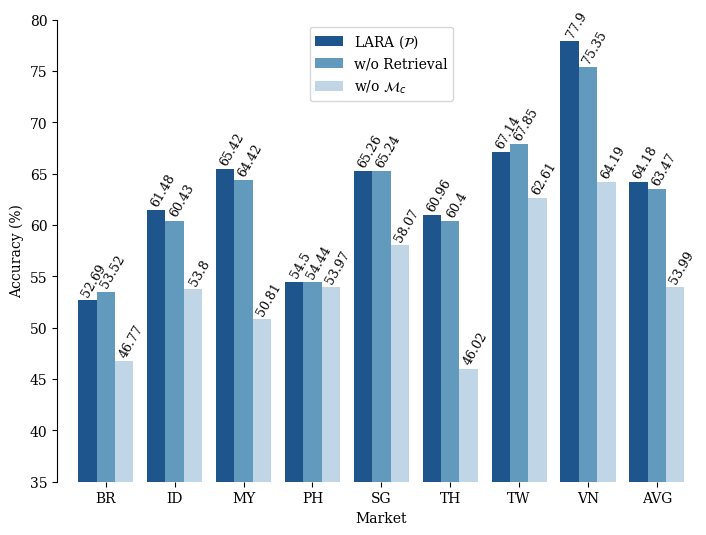
\includegraphics[width=.48\textwidth]{Figures/ablation_results.png}
    \vspace{-1cm}
    \caption{Ablation on different components of LARA.}
    \label{fig:ablation}
    \vspace{-0.3cm}
\end{figure}

\subsection{The role of retrievers in ICL retrieval}
% Demonstration selection could also have impact on the performance. Thus, we also tried to remove the retrieval component, and randomly sample the demonstrations for each intent. The results are reported with 10 runs on the random sampling. Based on Figure $\ref{fig:ablation}$, the overall performance will be worse if there is no retrieval component, specifically when there is a big demonstration pool or a high number of intents. Thus, if there is no one good strategy in pruning the demonstration pool, the easier way is to retrieval demonstrations based on their similarity to the task input.
% !-- to replace the part above --!
Demonstration selection via retrievers may have an impact on the performance. Thus, we remove all retrievers and randomly sample the demonstrations for each intent. The results are reported with 10 runs on the random sampling. As shown in Figure $\ref{fig:ablation}$, the overall performance decreased by 0.71\% without retrievers, highlighting the importance of selecting demonstrations which are more similar to test queries. ID and VN, with demonstration pool two to three times bigger than others (refer to Appendix \ref{appendix:b} for pool size), are affected the most because the chance of selecting samples which are not so similar is higher. 


\subsection{Quality of Embedding Model}
We also experimented with open-source, multilingual semantic similarity models provided by SentenceTransformers \cite{reimers-2019-sentence-bert} for in-context demonstration mining. These models are easily accessible to the public and cover a wide range of languages. Due to the training method, the similarity metric used is still cosine similarity.

The multilingual models selected in this experiment have lower or roughly the same number of parameters as our own XLM-RoBERTa-base model used in the paper. They are
\begin{itemize}
   \item \textbf{Models with all-rounded abilities} which have the best average performance reported by the authors: \textit{all-MiniLM-L12-v2} and \textit{all-mpnet-base-v2}
   \item \textbf{Models for paraphrase mining} as it is similar to our task of comparing multi-turn utterances to single-turn utterances: \textit{paraphrase-multilingual-MiniLM-L12-v2} and \textit{paraphrase-multilingual-mpnet-base-v2}
\end{itemize}

All comparisons are done using the same prompt, $\mathcal{P}_{formatted}$. From the table \ref{table:results_encoder}, the best open-source model of selections (from row 2 - 5) is overall only 0.35\% behind our own model, which means that the quality of the embedding model does not matter much and can easily be replaced by open-source models. That said, we would recommend paraphrase mining models over the general purpose ones as they are more suited for the scenario. Furthermore, if resource is a concern, smaller models like \textit{MiniLM-L12} can be selected with 3x speed up compared to \textit{mpnet-base}, all while maintaining the same overall quality.